% 摘要页沿用 draft/D题 的矢量页眉，已从原页眉移除具体论文题目。
% 题目在原位置使用同一工程的宋体字号叠加；正文参数来自原 sections/abstract.tex。
\newenvironment{paperabstractpage}[1]{%
  \clearpage
  \newgeometry{left=70.8bp,right=69.676bp,top=70.8bp,bottom=91.29bp,footskip=34.2bp}%
  \begingroup\normalfont\songti\fontsize{12bp}{20.28bp}\selectfont
  \setlength{\parindent}{24bp}\setlength{\parskip}{0pt}\setlength{\topskip}{12bp}%
  \AddToShipoutPictureBG{\AtPageLowerLeft{
\includegraphics[width=\paperwidth,height=\paperheight]{assets/abstract-continuation.pdf}}}%
  \AddToShipoutPictureBG*{%
    \AtPageLowerLeft{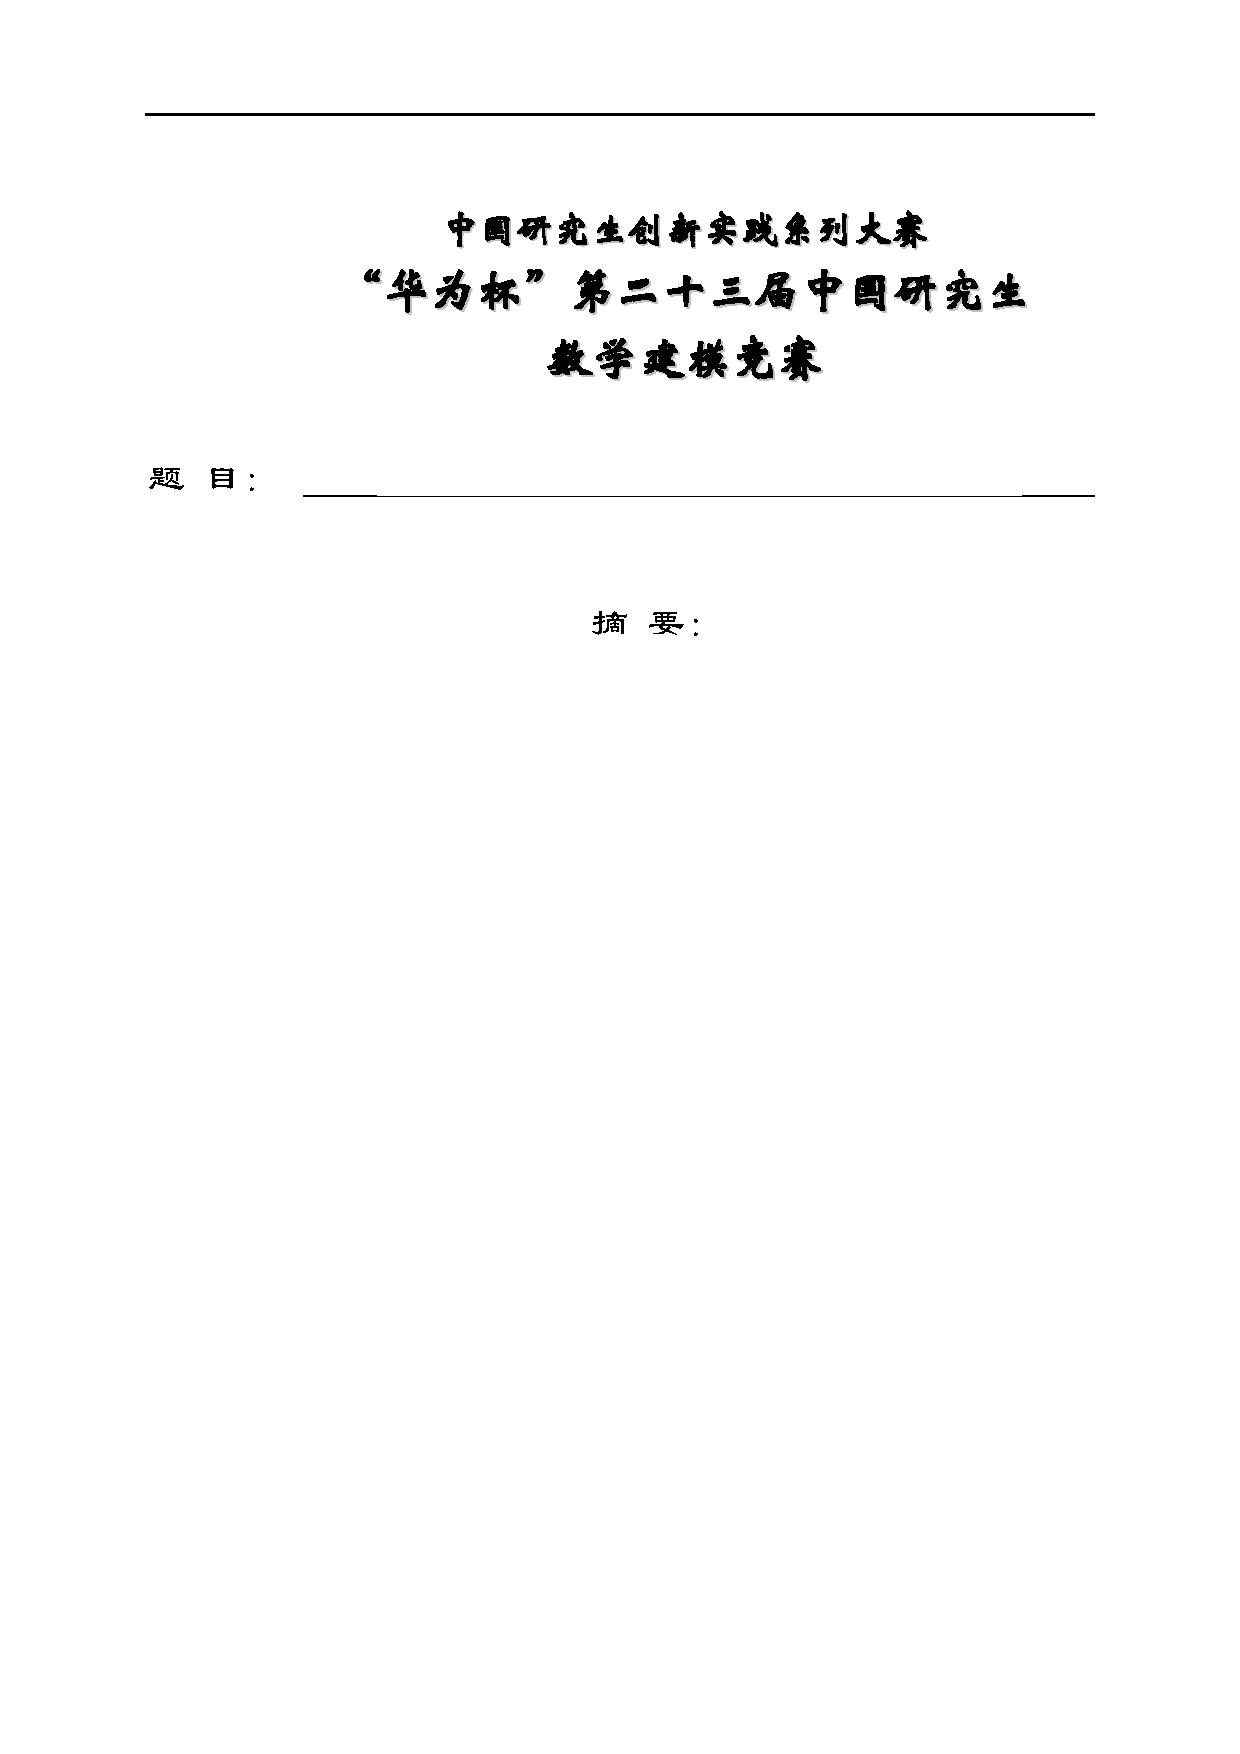
\includegraphics[width=\paperwidth,height=\paperheight]{assets/abstract-header.pdf}}%
    \AtPageUpperLeft{\put(181.8bp,-235.185bp){\heiti\fontsize{16.2bp}{18bp}\selectfont #1}}%
  }%
  \vspace*{231.12bp}%
}{%
  \par\clearpage\ClearShipoutPictureBG\endgroup\restoregeometry
}
\newcommand{\paperabstractkeywords}[1]{%
  \par\vspace{20.28bp}\noindent
  {\CJKfamily{abstractlisu}\fontsize{18bp}{20.28bp}\selectfont 关键词：}#1\par}
